\documentclass[11pt,a4paper]{article}
\usepackage[utf8]{inputenc}
\usepackage[T1]{fontenc}
\usepackage{lmodern}
\usepackage[ngerman]{babel}
\usepackage{graphicx}
% \usepackage{babelbib}
\usepackage{hologo}
\usepackage{csquotes}
\usepackage{amsmath}
\usepackage{amssymb}
\usepackage{amsthm}
\usepackage{biblatex}
\usepackage{listings}
\usepackage{xcolor}
\lstset{basicstyle=\ttfamily}
\addbibresource{literature.bib}

\hyphenation{Ku-ber-ne-tes}
\hyphenation{Ma-ni-fest}
% \hyphenation{Ser-vice}


\definecolor{codegreen}{rgb}{0,0.6,0}
\definecolor{codegray}{rgb}{0.5,0.5,0.5}
\definecolor{codepurple}{rgb}{0.58,0,0.82}
\definecolor{backcolour}{rgb}{0.95,0.95,0.95}

\lstdefinestyle{mystyle}{
    backgroundcolor=\color{backcolour},   
    commentstyle=\color{codegreen},
    keywordstyle=\color{magenta},
    numberstyle=\tiny\color{codegray},
    stringstyle=\color{codepurple},
    basicstyle=\ttfamily\footnotesize,
    breakatwhitespace=false,         
    breaklines=true,                 
    captionpos=b,                    
    keepspaces=true,                 
    numbers=none,                    
    numbersep=5pt,                  
    showspaces=false,                
    showstringspaces=false,
    showtabs=false,                  
    tabsize=2
}

\lstset{style=mystyle}
\title{Container-Management-Tool Kubernetes}
\begin{document}
% \maketitle

\tableofcontents
\thispagestyle{empty}
\newpage

% \section{Zusammenfassung}
% Kubernetes bietet als weit verbreitetes Container-Orchestrierungs-Tool vielfältige Möglichkeiten.
% Diese Arbeit ordnet Kubernetes und die zugrundeliegende Motivation in einen historischen Kontext ein. 
% Darauf aufbauend werden wichtige Komponenten und deren Verwendung beschrieben und erklärt.
% Zur Illustration wird ein Anwendungsfall aus dem Bereich des Data Farmings verwendet, 
% bei dem ein Simulationsmodell zur Optimierung der Einsatzbereitschaft einer Fahrzeugflotte mit den 
% durch Kubernetes zur Verfügung gestellten Komponenten skalierbar betrieben wird. Dieses Simulationsmodell
% gliedert sich in eine Microservice-Architektur ein, die Bedienung und Auswertung der Simulation erlaubt, 
% sowie Mittel zur Speicherung von Konfigurationen und Ergebnissen bietet.
% Im Ergebnis zeigt sich Kubernetes als geeignet, um sowohl die Simulation als auch die notwendigen 
% Stützservices skalierbar zu betreiben.
% Dennoch werden auch Limitationen diskutiert, die zum Teil durch fehlende 
% Hardware-Ressourcen aber auch durch die Komplexität von Kubernetes entstehen können.
% Abschließend folgt ein Ausblick über die mögliche Weiterentwicklung des Anwendungsfalls
% an sich und die zu erwartende Entwicklung von Kubernetes im Allgemeinen in den nächsten Jahren.


\clearpage
\pagenumbering{arabic}
\section{Einleitung}
\label{sec:einleitung}
Diese Arbeit soll einen Überblick über das Container-Orchestrierungs-Tool \emph{Kubernetes} geben.
Dazu werden zunächst Historie und grundlegende Funktionsprinzipien von Kubernetes beschrieben.
In dem darauffolgenden Kapitel wird aufgeführt, wie Kubernetes in Verbindung mit modernen
Konzepten zur Entwicklung und zur Ausbringung von Software genutzt werden kann,
um diese Prozesse zu beschleunigen und zu vereinfachen.
Anhand von Fallbeispielen bekannter Unternehmen, die Kubernetes in ihre Infrastruktur übernommen haben,
werden die Möglichkeiten zur praxisnahen Nutzung von Kubernetes skizziert.
Die Arbeit schließt mit einem Fazit zu den Eigenschaften, Vor- und Nachteilen
von Kubernetes sowie einem Ausblick zur erwarteten zukünftigen Rolle von Kubernetes
in Wirtschaft und Forschung.

Zunächst soll die Historie betrachtet werden, vor deren Hintergrund Kubernetes entstanden ist.
Das stetige Ziel, das sich durch diese Historie zieht, ist das Bereitstellen von Anwendungen.
Kominos et al. \cite{7899247} beschreiben die 1960er Jahre als Ursprung des Cloud-Computings.
Zu dieser Zeit liefen Anwendungen oft auf einer gemeinsamen Hardware und die Ressourcenverteilung erfolgte unmittelbar durch das zugrundeliegende Betriebssystem.
Ein derartiges Szenario (auch als „Bare-Metal“ bezeichnet) bringt in der Regel mehrere Herausforderungen mit sich.
Zum einen kann es schnell zu Abhängigkeitskonflikten zwischen den verschiedenen Anwendungen geben.
Ist eine Anwendung darauf angewiesen eine bestimmte Abhängigkeit in der Version <1.4 zu nutzen und eine andere
benötigt eine Version \(\geq 1.4\) derselben Abhängigkeit, lässt sich das nur schwer vereinbaren.
Zum anderen erschwert dieser Aufbau eine effiziente Ressourcenverteilung. Selbst wenn eine Anwendung alleine auf einem Rechner betrieben wird (z.B. um Konflikte zu anderen
Anwendungen zu vermeiden), muss dieser Rechner ausreichende Kapazitäten haben, um die höchsten Anfragespitzen an diese Anwendung zu verarbeiten.
Selbst dann, wenn diese Anfragespitzen nur äußerst selten erreicht werden \cite{Schmeling_Dargatz_2022} (S. 115-116).

Eine Weiterentwicklung dieser Bare-Metal-Architektur waren virtuelle Maschinen.
Virtuelle Maschinen erlauben es, auf derselben Hardware mehrere virtuelle Instanzen eines
Systems zu nutzen. Die Instanzen nutzen dabei nicht direkt die physischen Ressourcen, sondern lediglich virtuelle,
die durch Software nachgebildet werden.
Dadurch, dass verschiedene Anwendungen in verschiedenen virtuellen Maschinen betrieben werden, können Abhängigkeitskonflikte zwischen Anwendungen
vermieden werden. Weiterhin sind virtuelle Maschinen leichter auszubringen und zu administrieren als Bare-Metal-Lösungen.
Grundsätzlich können mit diesem Ansatz Anwendungen auch flexibler und skalierbarer bereitgestellt werden.
Leistungsfähige Hardware kann Anfragespitzen einer Anwendung in einer virtuellen Maschine abfangen und
zu anderen Zeiten anderen virtuellen Maschinen mit anderen
Anwendungen diese Ressourcen zuweisen.
Obwohl das schon einige Verbesserungen im Vergleich zu Bare-Metal-Lösungen sind, haben auch virtuelle Maschinen ihre eigenen Limitationen.
Da virtuelle Maschinen jeweils Ressourcen für ein eigenes Betriebssystem beanspruchen, geht vergleichsweise viel Leistung verloren,
die besser in der Anwendung genutzt werden könnte \cite{kofler2021docker} (S. 48).

Die nächste Stufe der Weiterentwicklung waren (Software-)\emph{Container}. Container haben einige Gemeinsamkeiten mit virtuellen Maschinen, doch der wesentliche Unterschied ist,
dass Container deutlich leichtgewichtiger sind. Das wird unter anderem dadurch erreicht, dass sie, statt ein komplett eigenes Betriebssystem zu verwenden,
Anteile des Host-Betriebssystems mitnutzen. Dadurch sind die „Baupläne“ (sog. Images) für Container im Allgemeinen kleiner als für klassische virtuelle Maschinen.
Durch den verringerten Overhead können auf gleicher Hardware auch mehr Container parallel betrieben werden, als es mit virtuellen Maschinen möglich wäre.
Insgesamt können mit Containern Leistungswerte erreicht werden, die die von virtuellen Maschinen deutlich übertreffen,
und nahezu an die von Bare-Metal heranreichen \cite{1272998.1273025}.
Durch diesen Umstand und dadurch, dass Container meist innerhalb weniger Sekunden gestartet werden können, sind diese besonders geeignet,
um flexibel auf unterschiedliche Anfrageintensitäten zu reagieren und Ressourcen effizient zu verteilen \cite{kofler2021docker} (S. 48).

Container eignen sich besonders, um \emph{Microservice-Architekturen} zu betreiben \cite{7158965}. Dabei handelt es sich um die
Entwicklung von Anwendungen, indem sie in kleine, unabhängige (Micro-)Services aufgeteilt werden. Jeder Microservice gehört zu
einem eigenen Prozess und die Kommunikation untereinander erfolgt durch leichtgewichtige Protokolle \cite{8406008}.
Der Vorteil von Microservice-Architekturen liegt im Vergleich zu monolithischen Architekturen in der
leichteren Skalierbarkeit einzelner Module und darin, dass Services weitgehend unabhängig voneinander
ausgebracht werden können. Zusätzlich erlauben sie, dass einzelne Services in unterschiedlichen Programmiersprachen
verfasst sein können sogar von unterschiedlichen Teams entwickelt werden \cite{microservices}.

Andererseits bringen Microservice-Architekturen im Vergleich zu monolithischen Anwendungen
auch neue Herausforderungen mit sich.
Grundsätzlich ist es komplexer eine Microservice-Architektur aufzubauen.
Dazu gehört insbesondere, zu definieren, aus welchen Microservices eine Anwendung bestehen soll
und welche Aufgaben diese jeweils umfassen. Darüber hinaus kann das Testen von Microservice-Architektur
herausfordernd sein \cite{8406008}.

Abbildung \ref{fig:arch-vergleich} visualisiert exemplarisch, welche Ebenen bei Bare-Metal-Architekturen, virtuellen Maschinen und Containern
jeweils zwischen Hardware und den Anwendungen liegen und wie Anwendungen voneinander isoliert werden.

\begin{figure}[h]
  \centering
  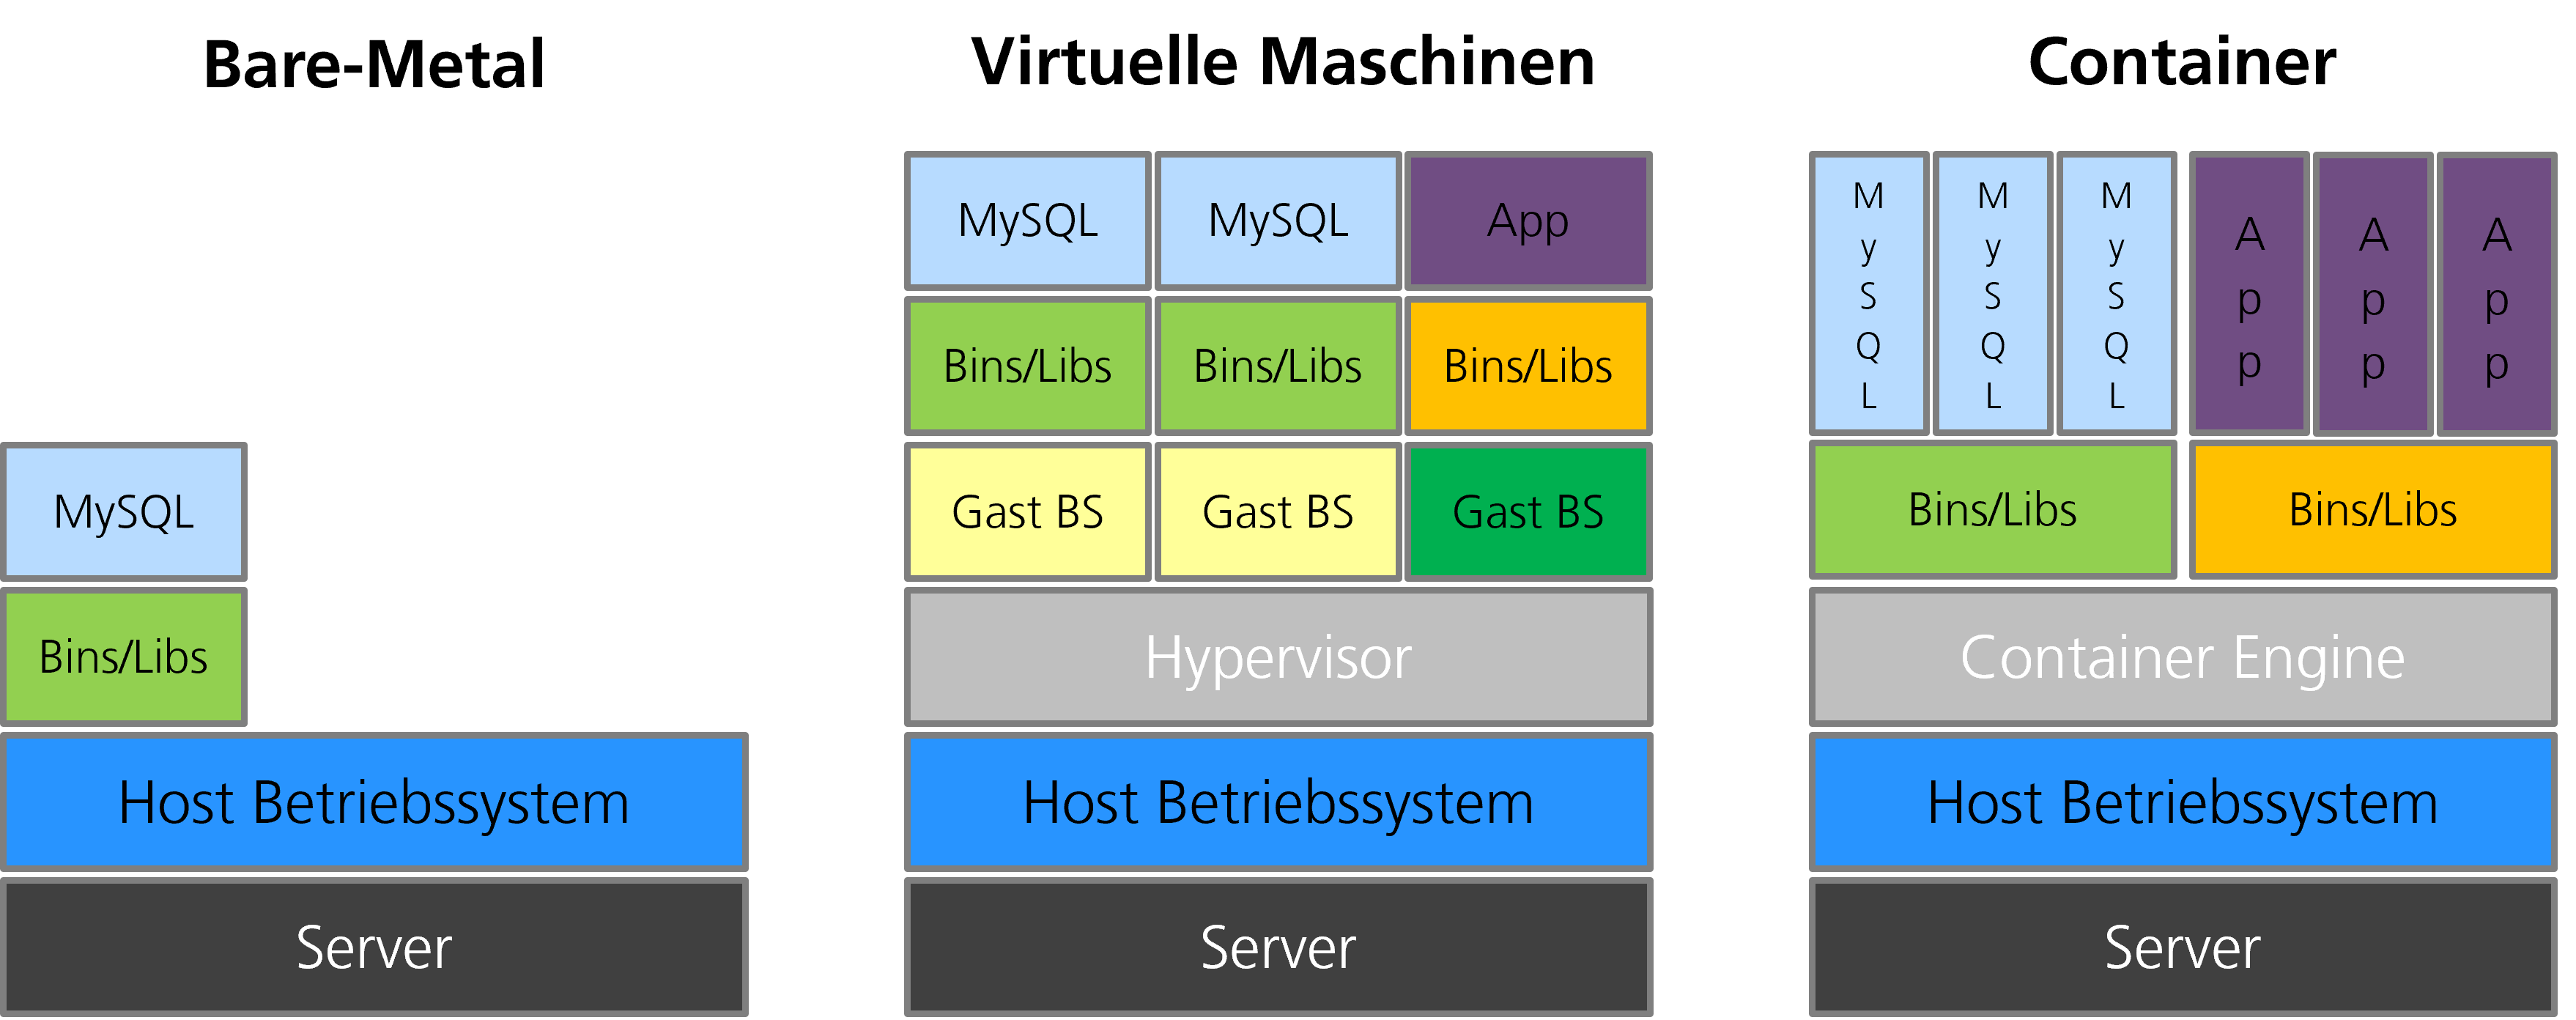
\includegraphics[width=1\textwidth]{./media/7899247 (eigen).png}
  \caption{Eine Gegenüberstellung von Bare-Metal-Architekturen, virtuellen Maschinen und Containern zeigt die einzelnen Ebenen und die Trennung von Anwendungen \cite{7899247}.}
  \label{fig:arch-vergleich}
\end{figure}

Kubernetes bietet als eines der heute populärsten Tools zur Orchestrierung von Containern
diverse Möglichkeiten, um vor allem containerisierte Microservice-Architekturen effizient zu verwalten.
Es abstrahiert dazu von allen beteiligten Rechnern und deren Ressourcen und bietet zentrale Steuerungsmöglichkeiten
\cite{Schmeling_Dargatz_2022} (S. 1) \cite{cicd_with_kubernetes_devops} (S. 10).

Kubernetes ist eine Software, die sich der Ausbringung (Deployment), der Skalierung und der Überwachung (Monitoring) von Containern widmet.
Dieser Vorgang wird auch als Container-Orchestrierung oder als Container-Management bezeichnet \cite{Bisong2019} (S. 664).
In diesem Zusammenhang wird Kubernetes auch als \emph{Betriebssystem der Cloud} bezeichnet \cite{Schmeling_Dargatz_2022} (S. 4).
Entwickelt wurde Kubernetes von Google. Dort wurde seit den frühen 2000er Jahren ein selbst entwickeltes Container-Management-System namens \emph{Borg} genutzt,
um Googles Services möglichst performant zu betreiben.
Im Jahr 2013 wurde \emph{Borg} von dessen Nachfolger \emph{Omega} abgelöst. Im selben Jahr erschien auch Docker, was ein wesentlicher Baustein des Kubernetes
Projekts werden sollte \cite{ibm_history}.

Die drei bei Google beschäftigten Ingenieure Craig McLuckie, Joe Beda und Brendan Burns setzten sich damals dafür ein,
die bei \emph{Borg} und \emph{Omega} gemachten Erfahrungen zu nutzen, um ein leichter bedienbares Container-Orchestrierungs-Tool
mit nutzerfreundlicher Schnittstelle zu entwickeln \cite{ibm_history}.

2014 wurde Kubernetes als eine Open-Source-Variante von \emph{Borg} \cite{43438} veröffentlicht und schließlich 2015 mit der Veröffentlichung von Kubernetes 1.0
von Google an die Cloud Native Computing Foundation (CNCF, \lstinline|https://www.cncf.io/|) gespendet. In den folgenden Jahren wuchs der Nutzerkreis von Kubernetes
rasch an und es konnte sich deutlich gegen konkurrierende Anwendungen durchsetzen.
Heutzutage ist Kubernetes, nach Linux, das zweitgrößte Open-Source-Projekt der Welt und wird von 71 \% der Fortune 100 Unternehmen genutzt
\cite{ibm_history} \cite{kubernetes_journey}.
Auf der Kubernetes Website wird es als ein Open-Source System für automatisierte Ausbringung, Skalierung
und Steuerung von containerisierten Anwendungen beschrieben \cite{kubernetes.io_start}.

Im Folgenden soll die Funktionsweise von Kubernetes beschrieben und schließlich anhand eines Beispiels
verdeutlicht werden.

\section{Container}
\label{sec:Container}

Für die Technologie von Containern haben sich mit der Zeit mehrere Alternativen entwickelt, die unterschiedliche
Stärken und Schwächen aufweisen. Zum einen gibt es die Technologien \emph{Singularity} und \emph{uDocker}, deren Stärken
vor allem in wissenschaftlichen Anwendungen über verteilte Rechenressourcen wie zum Beispiel High-Performance Computing
liegen. Zum anderen gibt es die Technologie \emph{Docker}, die sich als die heutzutage populärste Containertechnologie
herausgestellt hat und daher auch für die folgenden Kapitel als Grundlage angenommen wird \cite{Bentaleb_Belloum_Sebaa_El-Maouhab_2021}.

Um den Begriff des (Docker-)Containers zu verstehen, wird zunächst der Begriff \emph{Image} benötigt.
Ein Image kann wie in der Einleitung bereits beschrieben als eine Art Bauplan für einen Container gesehen werden.
Es stellt ein read-only Dateisystem als Basis für den Container zur Verfügung. Der Container nimmt an seinem Image
keine Änderungen vor. Stattdessen wird jedes Hinzufügen und jede Änderung während der Laufzeit des Containers in einem
getrennten Overlay-System behandelt.
Das heißt, dass diese Änderungen in einem Verzeichnis auf dem Host-System abgebildet werden.
Dadurch können beliebig viele Container von demselben Image abgeleitet werden \cite{kofler2021docker} (S. 140).
Eine Visualisierung dieses Konzepts ist in Abbildung \ref{fig:overlay} dargestellt.

\begin{figure}[h]
  \centering
  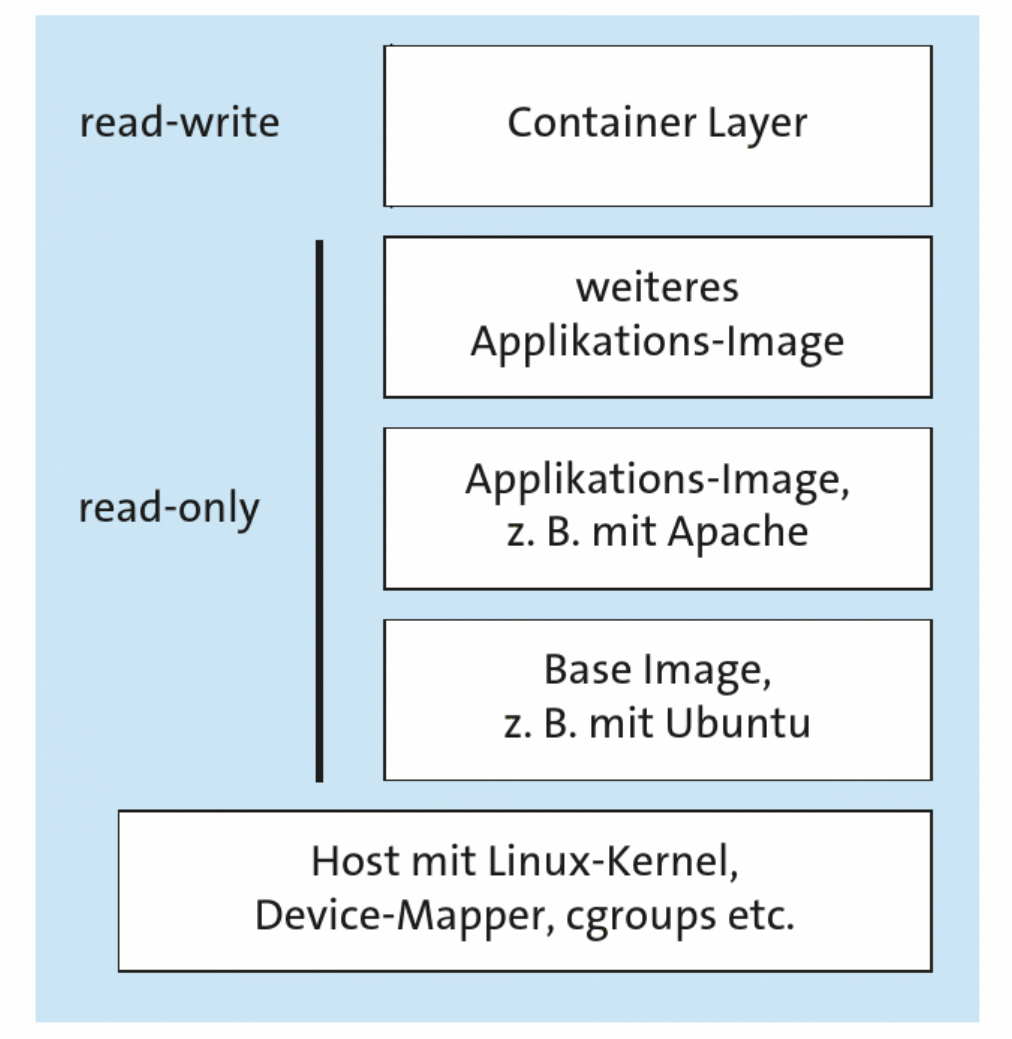
\includegraphics[width=0.5\textwidth]{./media/kofler2021docker S.140.png}
  \caption{Ein von einem Image abgeleiteter Container hat ein eigenes Dateisystem für Lese- und Schreibvorgänge, das
    von dem Dateisystem des Images getrennt ist \cite{kofler2021docker} (S. 140).}
  \label{fig:overlay}
\end{figure}

Für viele populäre Anwendungen gibt es vorgefertigte Images, die kostenfrei aus im Internet verfügbaren
\emph{Container-Repositories} (zum Beispiel \lstinline|https://hub.docker.com|) heruntergeladen werden können.
Darüber hinaus ist es auch möglich eigene Container-Repositories zu betreiben,
die zum Beispiel Images enthalten können, die von einem Unternehmen entwickelt wurden
und Dritten nicht zur Verfügung gestellt werden sollen.
Für einen konkreten Anwendungsfall kann es sinnvoll sein, ein bestehendes Basis-Image für die eigenen Zwecke anzupassen.
Dies ist mithilfe eines sogenannten \emph{Dockerfile}s möglich. Darin wird definiert, wie ein Base-Image z.B. durch das Hinzufügen von Dateien,
oder dem Ändern von Umgebungsvariablen angepasst werden soll. Dieses \emph{Dockerfile} wird dann für den \emph{build}
eines neuen Images verwendet \cite{kofler2021docker} (S. 81-82).

Aus dem erstellten Image können dann Container abgeleitet werden. Ein Container ist insofern „flüchtig“ als dass er nach seiner
Beendigung restlos gelöscht wird. Bei einem Neustart enthält er wieder nur die Daten, die vorher durch das Image definiert wurden.
Natürlich gibt es Anwendungsfälle, in denen die persistente Speicherung von Daten durch einen Container gewünscht ist, z.B. wenn
eine Datenbank in einem Container betrieben wird. Für diesen Fall gibt es das Konzept der \emph{Volumes}.
Ein Volume spiegelt einen definierten Speicherbereich aus dem Dateisystem des Containers auf das Host-System.
Wird ein Container beendet und durch einen neuen ersetzt, bindet dieser das Volume in sein Dateisystem ein übernimmt
dabei die Daten seines beendeten Vorgängers \cite{kofler2021docker} (S. 44-45).

Die in diesem Kapitel beschriebenen Konzepte sind ausreichend, um Container zu betreiben.
Nutzt man aber lediglich diese Konzepte, verhalten sich die Container im Prinzip wie leichtgewichtige virtuelle Maschinen.
Der eigentliche Vorteil von Containern, nämlich die horizontale Skalierbarkeit, wird damit noch nicht ausgenutzt.
Die \emph{horizontale} Skalierbarkeit ist abzugrenzen von der \emph{vertikalen} Skalierbarkeit.
Bei letzterer geht es darum, einen einzelnen Server um weitere Ressourcen (Rechenleistung, Speicher etc.) zu ergänzen.
Da hierbei keine Änderungen an der Anwendung selbst erforderlich sind, ist dieser Ansatz vergleichsweise leicht
zu administrieren. Er stößt jedoch schnell an seine physikalischen Grenzen und wird daher den hohen
Ressourcenanforderungen moderner Anwendungen oft nicht gerecht \cite{Schmeling_Dargatz_2022} (S. 64).

Horizontale Skalierung sieht im Gegensatz dazu vor, dass eine Anwendung
auf mehrere Rechner verteilt wird. Durch Hinzufügen weiterer Rechner können die zur Verfügung stehenden Ressourcen nahezu beliebig erweitert werden.
Zusätzlich ist auch eine geografische Optimierung möglich, indem zum Beispiel Server in der Nähe der erwarteten Clients platziert werden.
Letztendlich trägt horizontale Skalierung auch zur Ausfallsicherheit einer Anwendung bei, da der Ausfall einzelner Instanzen durch andere Instanzen
aufgefangen werden kann.
Container haben sich als eine wesentliche Grundlage für die horizontale Skalierung etabliert.
Der Nachteil dieser Methode ist die deutlich erhöhte Komplexität,
die mit dem Betrieb einer verteilten Anwendung einhergeht \cite{Schmeling_Dargatz_2022} (S. 64).

Im folgenden Kapitel soll beschrieben werden, welche Werkzeuge Kubernetes anbietet, um mit dieser Komplexität umzugehen.

\section{Grundlegende Kubernetes-Konzepte}
\label{sec:Grundlegende_Kubernetes-Konzepte}
Ein durch Kubernetes verwaltetes System wird üblicherweise als \emph{Cluster} bezeichnet.
Ein Cluster besteht aus einer oder mehreren physischen und/oder virtuellen Maschinen, die darin eingebunden sind.
Jede Maschine wird dabei als ein \emph{Node} (deutsch: Knoten) bezeichnet. Diese Nodes werden wiederum unterschieden in
\emph{Master Nodes} und \emph{Worker Nodes}.
Für viele Cluster reicht ein Master Node aus. In Hochverfügbarkeitsszenarien oder bei mehreren
tausend Worker Nodes kann es jedoch auch mehrere Master Nodes geben \cite{Schmeling_Dargatz_2022} (S. 7).
Wie die Namen vermuten lassen, ist der Master Node für die Orchestrierung
des Systems verantwortlich während die Worker Nodes bestimmte Aufgaben ausführen \cite{Bentaleb_Belloum_Sebaa_El-Maouhab_2021}.
Für den Spezialfall eines \emph{Single-Node-Clusters} kann dieser einzelne Node auch die Rolle von sowohl
Master als auch Worker übernehmen.

Master und Worker Nodes bestehen zur Erfüllung ihrer Aufgaben aus unterschiedlichen Komponenten,
die im Folgenden beschrieben werden.
Zur Veranschaulichung dieser Komponenten kann eine Containerschiffmetapher verwendet werden,
die in Abbildung \ref{fig:containerschiff} dargestellt ist. Dort gibt es mehrere Containerschiffe
(Worker Node 1 und 2), die ihre Anweisungen von einem Leitschiff (Master Node) erhalten \cite{Schmeling_Dargatz_2022} (S. 7).

Im Anschluss daran werden die wichtigsten Ressourcen
von Kubernetes beschrieben und anhand von kurzen Beispielen vorgestellt.

\begin{figure}[h]
  \centering
  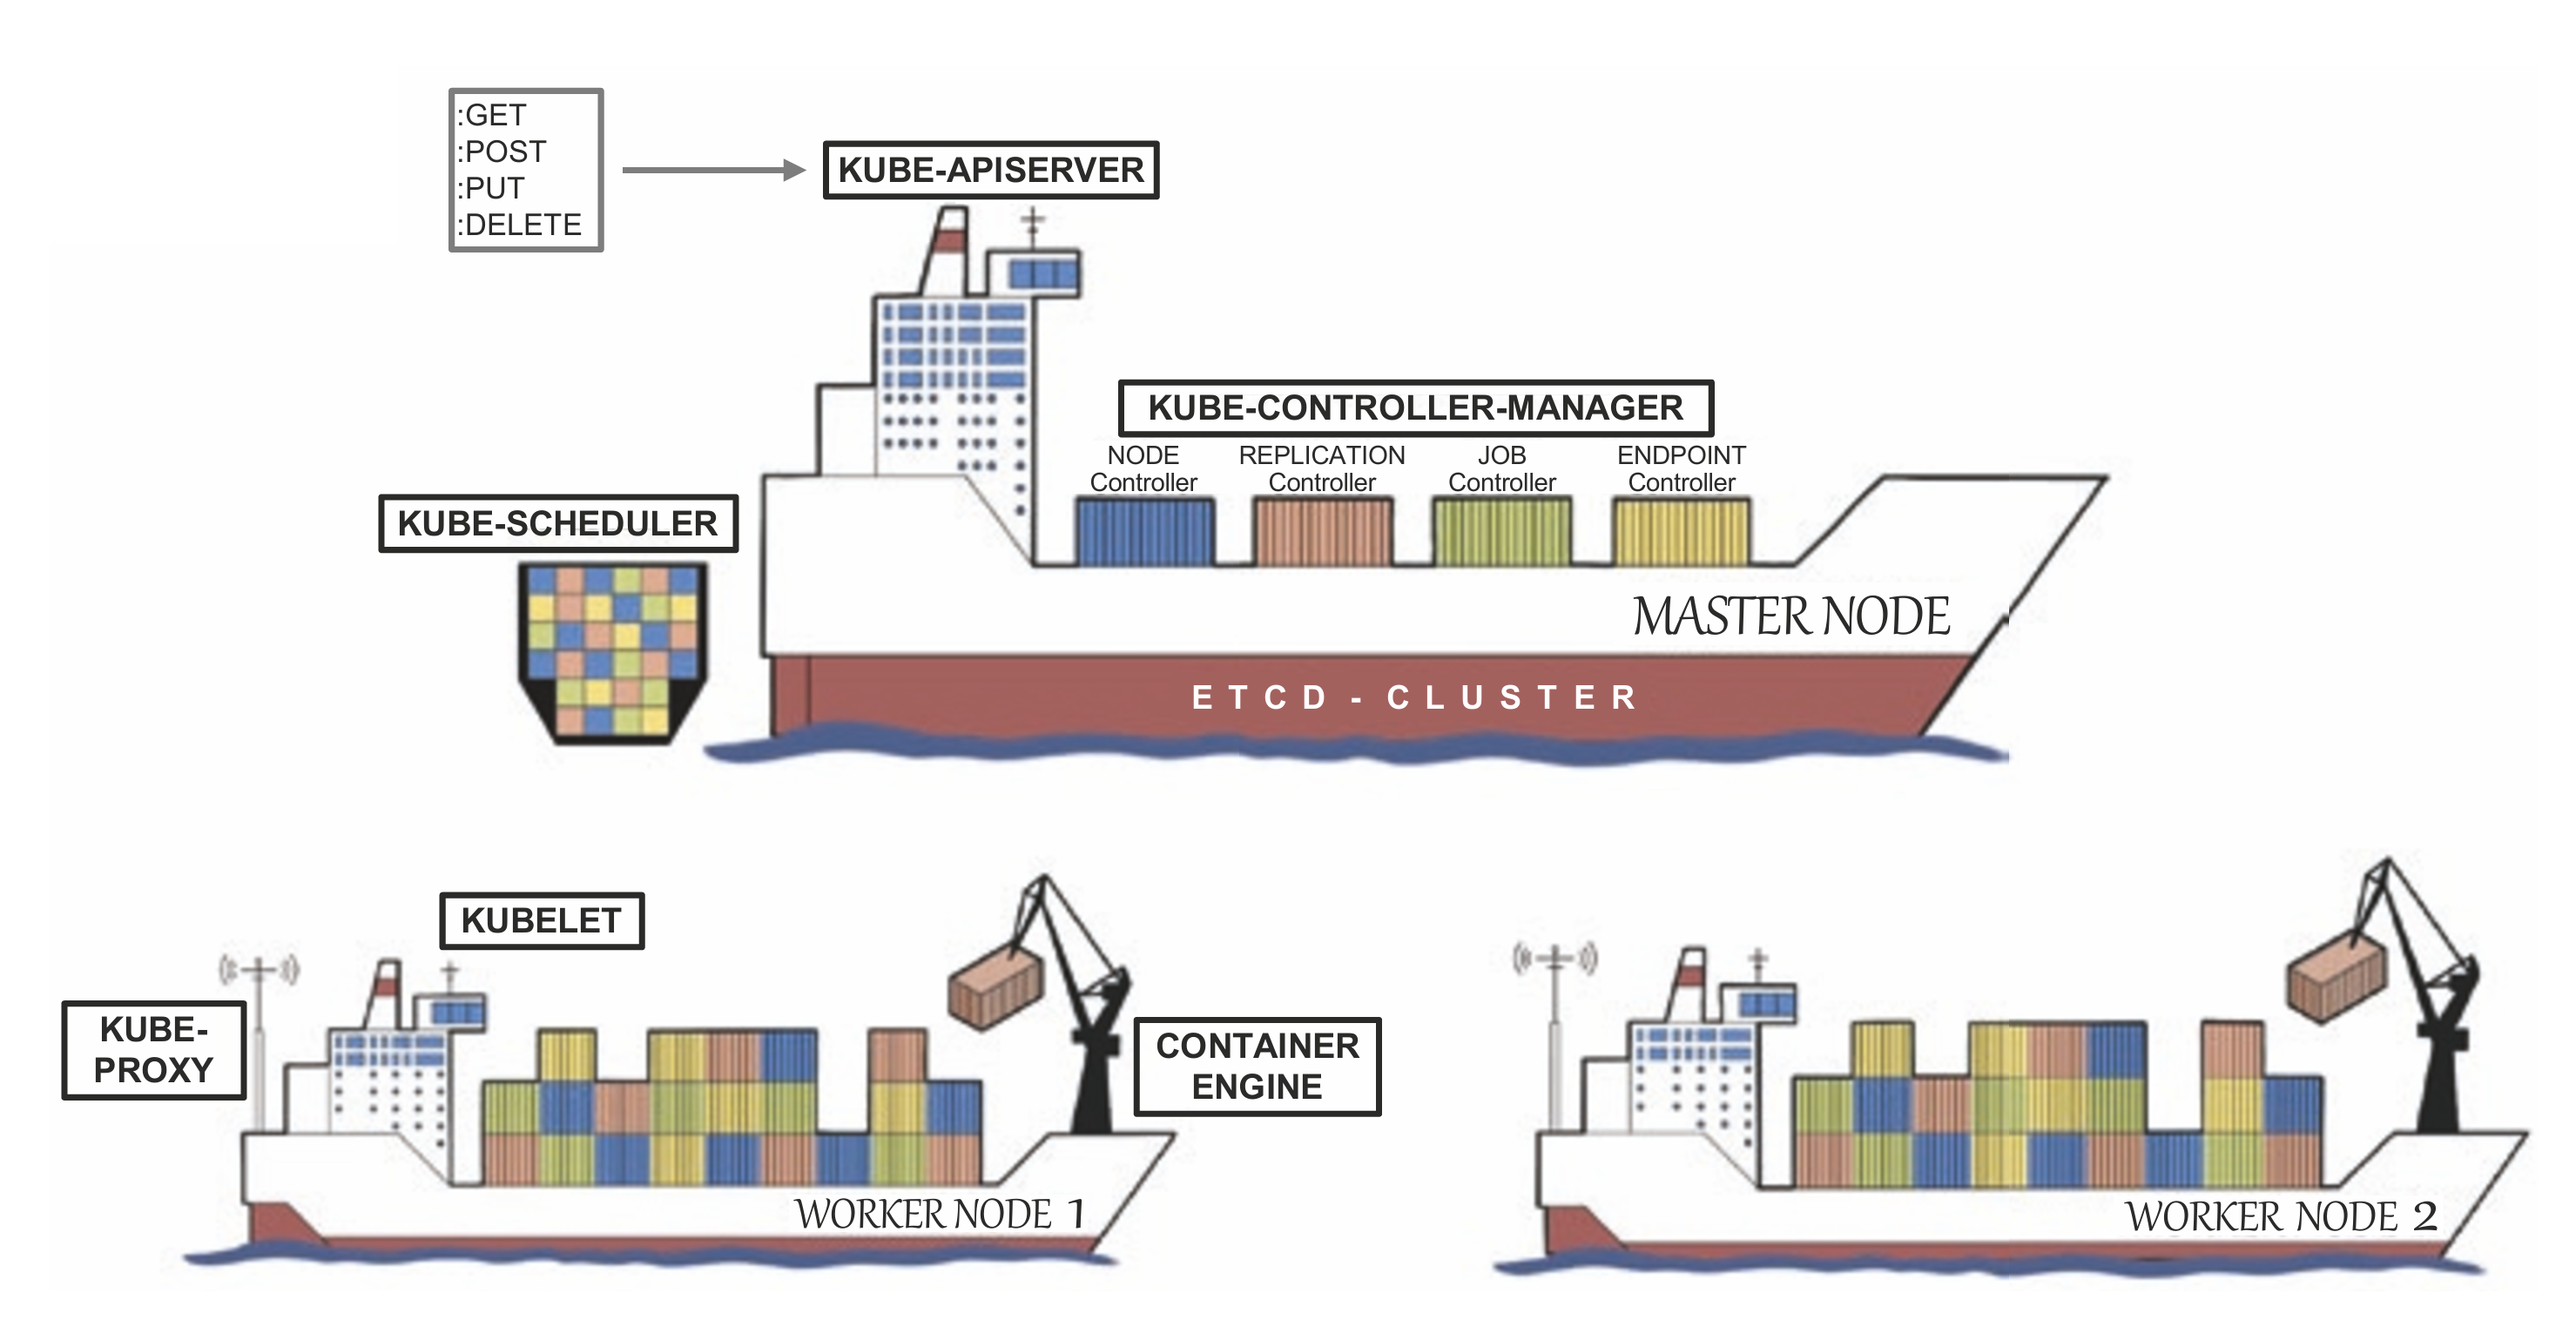
\includegraphics[width=1\textwidth]{./media/Schmeling_Dargatz_2022 S.7.png}
  \caption{Die verschiedenen Komponenten von Master und Worker Nodes können mit
    verschiedenen Komponenten eines Leitschiffs und mehrerer Containerschiffe verglichen werden. \cite{Schmeling_Dargatz_2022} (S. 7).}
  \label{fig:containerschiff}
\end{figure}

\subsection{Master Node Komponenten}
\label{sec:MasterNodeKomponenten}
Bei \emph{Etcd} handelt es sich um einen \emph{key-value-store} (Schlüssel-Wert-Speicher),
der alle Informationen über den Zustand eines Kubernetes Clusters speichert.
In Bezug auf die Containerschiffmetapher kann Etcd als das Logbuch des Schiffs verstanden werden.
Jede Änderung an den Cluster-Ressourcen wird im Etcd gespeichert und von dort wieder abgerufen.
Etcd wird auf jedem Master Node ausgeführt, wobei einer dieser Nodes als „Anführer“
ausgewählt wird und dieser die Schreibanfragen verarbeitet \cite{Schmeling_Dargatz_2022} (S. 8).

Die übliche Vorgehensweise um mit einem Kubernetes Cluster zu interagieren, ist das Kommandozeilenwerkzeug \emph{kubectl}.
Dieses Werkzeug ermöglicht sowohl die Abfrage als auch die Änderung von im Cluster vorhandenen Ressourcen.
Im Hintergrund stellt \emph{kubectl} eine Anfrage an den \emph{Kube-apiserver}, der Endpunkte anbietet,
um mit dem Cluster zu interagieren. Vergleichbar mit der Kommandobrücke des Leitschiffs ist der Kube-apiserver
somit dafür verantwortlich, die angefragten Informationen
aus verschiedenen Quellen zu sammeln und gegebenenfalls andere Komponenten anzuweisen, bestimmte Änderungen vorzunehmen \cite{Schmeling_Dargatz_2022} (S. 10).

Neben dem tatsächlichen Zustand des Clusters enthält Etcd auch den gewünschten Zustand.
Sollten diese voneinander abweichen, ist es die Aufgabe des \emph{Kube-Controller-Managers},
dies zu erkennen und über eine Anfrage an den Kube-apiserver den gewünschten Zustand wiederherzustellen.
Er überwacht also symbolisch mit Containerschiffe. \cite{Schmeling_Dargatz_2022} (S. 11).

Der \emph{Kube-Scheduler} entscheidet, welche Container auf welchem Node betrieben werden.
Im Sinne der Containerschiffmetapher ist dies die Komponente, die bestimmt
wie und wo welche Container verstaut werden.
Er verwaltet dazu Informationen über verfügbare Rechen- und Speicherressourcen sowie über weitere Eigenschaften
der Nodes \cite{Schmeling_Dargatz_2022} (S. 12).

\subsection{Worker Node Komponenten}
\label{sec:WorkerNodeKomponenten}
Auf jedem Worker Node finden sich drei wesentliche Komponenten.
Die erste Komponente ist der \emph{Kubelet}. Das Kubelet kann als Schnittstelle
zu den Master Nodes beziehungsweise als Kommandobrücke der Containerschiffe gesehen werden.
Sobald der Kube-Scheduler entschieden hat, auf welchem
Worker Node ein Container betrieben werden soll, bekommt das Kubelet auf diesem Node
vom Kube-apiserver den Auftrag einen Container zu starten \cite{Schmeling_Dargatz_2022} (S. 13).

Kubelet gibt diesen Auftrag weiter an die Komponente \emph{Container Runtime}, die
in Abbildung \ref{fig:containerschiff} als die Kräne der Containerschiffe dargestellt ist.
Diese übernimmt das eigentliche Starten des Containers, in dem sie das zugehörige Image
abruft (zum Beispiel von \lstinline|https://hub.docker.com|) und daraus einen Container erstellt \cite{Schmeling_Dargatz_2022} (S. 13).

Der physische „Standort“ eines Containers, also der Node, auf dem er betrieben wird, ist insofern
flüchtig, als das der Container jederzeit auf einem anderen Node neu ausgebracht werden könnte.
Um trotzdem einen Überblick zu behalten, welcher Container wo verortet ist, gibt es die Komponente
\emph{Kube-Proxy}. Auf jedem Node läuft genau eine Instanz des Kube-Proxys \cite{Schmeling_Dargatz_2022} (S. 14).

\subsection{Clusterinitialisierung}
Um die Ressourcen zu verwenden, muss zunächst ein Cluster aufgesetzt werden.
Im Rahmen dieser Arbeit wird dazu \emph{Minikube} verwendet.

Minikube ist eine Anwendung, die genutzt werden kann, um mit vergleichsweise wenig Aufwand ein lokales
Kubernetes Cluster mit einem Node zu erstellen, das für Test- und Entwicklungsaufgaben genutzt werden kann.
Zum Betrieb des Clusters verwendet Minikube eine virtuelle Maschine, innerhalb derer
alle Kubernetes Komponenten laufen. Dementsprechend ist eine der Voraussetzungen,
um Minikube zu nutzen auch die vorherige Installation einer Virtualisierungsanwendung.
Näheres kann der Minikube Dokumentation entnommen werden \cite{minikube}.

\subsection{Pods}
\emph{Pods} sind die kleinste adressierbare Einheit in einem Kubernetes Cluster.
Sie sind die Entitäten, innerhalb derer der Anwendungscode ausgeführt wird.
Im Kapitel \ref{sec:WorkerNodeKomponenten} wurde beschrieben, dass Container auf Nodes betrieben werden.
Diese Darstellung ist allerdings nur indirekt richtig. Tatsächlich werden nicht Container,
sondern Pods auf Nodes betrieben.
Ein Pod wiederum kann einen oder mehrere Container enthalten. Enthält ein Pod nur einen Container,
kann dieser als einfacher „Wrapper“ für diesen verstanden werden.
Wenn ein Pod mehrere Container enthält, teilen sich diese eine IP-Adresse,
den Port-Space, den Hostnamen und ein gemeinsames Dateisystem.
Zusätzlich bedeutet es, dass diese Container nur gemeinsam skalierbar sind.
Das bietet sich in der Regel dann an, wenn die Funktionen dieser Container eng gekoppelt sind und eine Instanz eines
Containers nur dann sinnvoll zu betreiben ist, wenn auch ihr „Partner-“Container vorhanden ist \cite{9783969109625} \cite{Schmeling_Dargatz_2022} (S. 18-19).

Ein Beispiel für die Nutzung mehrerer Container innerhalb eines Pods ist die Verwendung
eines zusätzlichen „Sidecar-Containers“, der den Pod einer Anwendung um ein Netzwerkmanagement erweitert \cite{9783969109625}.

Ressourcen werden in Kubernetes meist in Form von \emph{.YAML-Dateien} definiert,
die auch als \emph{Kubernetes Manifeste} bezeichnet werden.
Eine mögliche minimale Konfiguration könnte beispielsweise wie in Listing \ref{lst:pod-config} aussehen.

\lstinputlisting[caption={Ein beispielhaftes Kubernetes Manifest zur Konfiguration eines Pods \cite{Schmeling_Dargatz_2022} (S. 20).}, label=lst:pod-config]{../kubernetes/nginx/pod.yaml}

Ein Kubernetes Manifest ist hierarchisch aufgebaut
und enthält stets die gleichen vier übergeordneten Schlüssel.
Die \emph{apiVersion} gibt an welche Version der Endpunkte des Kube-apiservers für diese Ressource
verwendet werden soll (vgl. \ref{sec:MasterNodeKomponenten}).
Der Schlüssel \emph{Kind} gibt an, um welche Art von Ressource es sich handelt.
In diesem Fall handelt es sich um einen Pod.
Unter dem Schlüssel \emph{metadata} wird zum einen ein Name für den Pod
und zum anderen eine Menge von frei wählbaren Labels definiert.
Schließlich werden unter \emph{spec} die inhaltlichen Spezifikationen des Pods
definiert. Für dieses Beispiel enthält der Pod nur einen Container, der ebenfalls den Namen
\emph{webserver} trägt. Das für den Container verwendete nginx Image \cite{nginx} wird aus einer
öffentlichen Container Registry in der Version 1.20.1 geladen. Da diesbezüglich keine weiteren
Einschränkungen gemacht werden, wird standardmäßig \linebreak \lstinline|https://hub.docker.com| als Container Registry
verwendet. Abschließend wird der Container über den Port 80 erreichbar gemacht \cite{Schmeling_Dargatz_2022} (S. 18-21).

Vorausgesetzt das Cluster ist bereits initialisiert, kann mit dem Kommandozeilenbefehl
\lstinline|kubectl create -f <Pfad/zum/Manifest>|
ein Pod mit dem Namen \emph{webserver} gestartet werden.

Über das Kommando \lstinline|kubectl get pod webserver| kann kontrolliert werden,
ob der Pod erfolgreich gestartet wurde. Eine mögliche Ausgabe ist in
Listing \ref{lst:pod-state} angegeben. Darin ist zu sehen, dass
von dem einen vorgesehenen Container im Pod \emph{webserver} auch einer vorhanden ist.
Der Status „Running“ zeigt an, dass der Pod einem Node zugewiesen und alle seine Container erstellt wurden.
Mindestens einer dieser Container läuft ebenfalls gerade oder wird gerade gestartet.
Weitere mögliche Zustände sind \cite{kubernetes.io_pod_lifecycle}:
\begin{itemize}
  \item \textbf{Pending}: Der Pod wurde erstellt, aber einer oder mehrere Container sind noch nicht gestartet.
  \item \textbf{Succeeded}: Alle Container im Pod haben ihre Ausführung erfolgreich beendet.
  \item \textbf{Failed}: Einer oder mehrere Container im Pod haben ihre Ausführung nicht erfolgreich beendet.
  \item \textbf{Unknown}: Der Status des Pods kann nicht ermittelt werden, normalerweise aufgrund eines Kommunikationsproblems mit dem Node.
\end{itemize}
Weiterhin wird angezeigt, dass noch kein Neustartversuch unternommen wurde
und der Pod seit 18 Sekunden existiert.
Bei Bedarf kann der Pod mit \lstinline|kubectl delete pod webserver| wieder gelöscht werden.

\begin{lstlisting}[caption={Der Pod wurde erfolgreich gestartet \cite{Schmeling_Dargatz_2022} (S. 21).}, label={lst:pod-state}]
NAME        READY   STATUS    RESTARTS   AGE
webserver   1/1     Running   0          18s
\end{lstlisting}

\subsection{ReplicaSets}
Pods bieten eine Grundlage, um Anwendungen flexibel zu gestalten und
transparent sowie reproduzierbar auszubringen \cite{Schmeling_Dargatz_2022} (S. 24-29).
Sofern aber nur einzelne Pods betrachtet werden, wird das Potenzial von Kubernetes
nicht vollständig ausgeschöpft.
Meist ist es beabsichtigt, Pods zu replizieren und gegebenenfalls
auf mehreren Nodes gleichzeitig zu betreiben.

Dazu stehen \emph{ReplicaSets} zur Verfügung.
In einem ReplicaSet ist definiert, welche Art von Pods (basierend auf einem gemeinsamen Image)
in welcher Konfiguration betrieben werden sollen. Zusätzlich wird hier festgelegt, wie viele \emph{Replikationen}
dieses Pods gleichzeitig vorhanden sein sollen.
Listing \ref{lst:rs-config} zeigt ein ReplicaSet, das drei Pods startet (Schlüssel \emph{replicas}).
Es ist zu beachten, dass die Konfiguration des ReplicaSets unabhängig von der Konfiguration
des Pods in Listing \ref{lst:pod-config} ist.
Die Spezifikationen welche Art von Pods in diesem ReplicaSet gestartet werden sollen,
erfolgt unter dem Schlüssel \emph{template} \cite{Schmeling_Dargatz_2022} (S. 26).
Wie auch schon bei den Pods kann dieses ReplicaSet mit dem Befehl
\lstinline|kubectl create -f <Pfad/zum/Manifest>| erstellt werden \cite{Schmeling_Dargatz_2022} (S. 24-29).

\lstinputlisting[caption={Ein beispielhaftes Kubernetes Manifest zur Konfiguration eines ReplicaSets mit drei Pods \cite{Schmeling_Dargatz_2022} (S. 26).}, label=lst:rs-config]{../kubernetes/nginx/replicaset.yaml}

Das Kommando \lstinline|kubectl get pods| erzeugt eine mit Listing \ref{lst:rs-pods}
vergleichbare Ausgabe. Dabei ist anzumerken, dass jeder Pod den Namen des ReplicaSets,
ergänzt um ein automatisch generiertes Suffix, erhält.

\begin{lstlisting}[caption={Drei Pods wurden erfolgreich gestartet \cite{Schmeling_Dargatz_2022} (S. 27).}, label={lst:rs-pods}]
NAME              READY   STATUS    RESTARTS   AGE
webserver-86mvm   1/1     Running   0          35s
webserver-bxvwp   1/1     Running   0          35s
webserver-wzrs8   1/1     Running   0          35s
\end{lstlisting}

Kompakter kann der Status des ReplicaSets mit dem Befehl \lstinline|kubectl get rs webserver|
abgerufen werden. Listing \ref{lst:rs-state} enthält eine mögliche Ausgabe.
Wird jetzt einer der Pods gelöscht, versucht der Kube-Controller-Manager automatisch
einen neuen Pod zu starten, um diesen zu ersetzen.

Das Replizieren von Anwendungen ist grundsätzlich kein neues Phänomen, aber
die wesentliche Neuerung durch Kubernetes ist, dass die Replikation einheitlich
und anwendungsunabhängig erfolgen kann \cite{Schmeling_Dargatz_2022} (S. 29).

\begin{lstlisting}[caption={Ein ReplicaSet mit drei erfolgreich gestarteten Instanzen \cite{Schmeling_Dargatz_2022} (S. 27).}, label={lst:rs-state}]
NAME        DESIRED   CURRENT   READY   AGE
webserver   3         3         3       8s
\end{lstlisting}

\subsection{Deployments}
\label{sec:Deployments}
Ein \emph{Deployment} ist ein Konzept, das im Schwerpunkt genutzt wird, um Änderungen an Anwendungen auszubringen.
Das Szenario, das ein Deployment notwendig macht, kann wie folgt beschrieben werden:

Eine Anzahl von Pods wurde im Rahmen eines ReplicaSets auf Basis eines gemeinsamen Images erstellt.
Es stellt sich heraus, dass das Image einen Fehler hat oder aus anderen Gründen aktualisiert werden muss.
Das ReplicaSet kann so konfiguriert werden, dass es zukünftig das neue Image für seine Pods verwendet.
Da die Pods aber bereits laufen, wird an diesen keine Änderung mehr vorgenommen. Es ist zwar möglich,
einzelne Pods zu löschen, die dann automatisch durch neue Pods, basierend auf dem neuen Image, ersetzt würden, aber
gerade mit steigender Anzahl an Pods ist dieser Prozess höchst
fehleranfällig, da es schwer zu überblicken ist, welche Pods noch mit dem alten und welche schon mit dem
neuen Image laufen. Alternativ könnten auch das gesamte ReplicaSet und damit alle zugehörigen Pods gelöscht werden.
Das kann in einer Testumgebung problemlos möglich sein. In einer Produktivumgebung möchte man derartige
Ausfälle aber in der Regel vermeiden \cite{Schmeling_Dargatz_2022} (S. 29-30).

Um diese Probleme zu bewältigen, kann ein Deployment erstellt werden.
Ein Deployment enthält wiederum ein ReplicaSet. Tritt nun das oben aufgeführte Szenario ein und ein Image
muss aktualisiert werden, reicht es, das Deployment dafür anzupassen.
Kubernetes stellt dann sicher, dass das alte ReplicaSet und die dazugehörigen Pods gelöscht werden.
Damit es dadurch aber keine Serviceunterbrechungen gibt, wird zunächst ein anderes ReplicaSet mit dem neuen
Image initialisiert. Während das alte ReplicaSet also schrittweise abgebaut wird, wird das neue ReplicaSet
schrittweise aufgebaut. Diese Strategie wird auch als \emph{Rolling Update} bezeichnet.
Ein Rolling Update kann so konfiguriert werden, dass immer eine bestimmte Mindestanzahl an
Pods während der Aktualisierung zur Verfügung steht.
Die Alternative zum Rolling Update ist die \emph{Recreate} Strategie, bei der zunächst
alle Pods der alten Version heruntergefahren werden, bevor die neuen gestartet werden.
Ein weiterer Vorteil von Deployments ist, dass sie anhand eines einzelnen Befehls auf die vorherige Version
zurückgesetzt werden können (sog. \emph{Rollback}). Das kann hilfreich sein, wenn sich nach Ausbringung eines
Updates herausstellt, dass dieses doch nicht den Erwartungen entspricht und man stattdessen bei der vorherigen
Version bleiben möchte \cite{Schmeling_Dargatz_2022} (S. 30-32).

Das Kubernetes Manifest für ein Deployment ist genauso aufgebaut, wie bereits beim ReplicaSet in
Listing \ref{lst:rs-config}, mit der Ausnahme, dass der Schlüssel \emph{kind} den Wert
\emph{Deployment} statt \emph{ReplicaSet} hat. Es kann auch ebenfalls mit dem Befehl
\lstinline|kubectl create -f <Pfad/zum/Manifest>| gestartet werden.
Dadurch wird ein Deployment erstellt, das wiederum ein ReplicaSet enthält.
Möchte man nun eine Änderung an dem Webserver vornehmen, beispielsweise indem
man ein aktuelleres Image verwendet, reicht es, den zugehörigen Wert im Manifest
zu verändern und anschließend mit \lstinline|kubectl apply -f <Pfad/zum/Manifest>| anzuwenden.
Listing \ref{lst:deploy-rollout} stellt dar wie durch mehrfaches Aufrufen
von \lstinline|kubectl get rs| sichtbar wird, wie das alte
ReplicaSet schrittweise abgebaut und das neue schrittweise aufgebaut wird \cite{Schmeling_Dargatz_2022} (S. 30-31).

Alternativ kann nach Initialisierung des Deployments die Anzahl der Replikationen auch mit
dem Befehl \lstinline|kubectl scale --replicas=<Anzahl Replicas> deployment/<Name des Deployments>|
verändert werden.

\begin{lstlisting}[caption={Ein Deployment, das schrittweise ein Update ausführt \cite{Schmeling_Dargatz_2022} (S. 31).}, label={lst:deploy-rollout}]
NAME                   DESIRED   CURRENT   READY   AGE
webserver-54596f9745   3         3         3       48s
webserver-57db766469   1         1         0       5s

NAME                   DESIRED   CURRENT   READY   AGE
webserver-54596f9745   2         2         2       53s
webserver-57db766469   2         2         1       10s

NAME                   DESIRED   CURRENT   READY   AGE
webserver-54596f9745   0         0         0       1m10s
webserver-57db766469   3         3         3       27s
\end{lstlisting}

\subsection{Services}
Innerhalb eines Kubernetes Clusters besteht ein internes Netzwerk. Dementsprechend hat auch jeder Pod
eine eigene IP-Adresse, über die er erreichbar ist. Diese IP-Adresse wird automatisch zugewiesen, wenn der Pod startet.
Auf diese Weise können Anwendungen innerhalb des Clusters über Pod-Grenzen hinweg miteinander kommunizieren.
Listing \ref{lst:pod-ip} zeigt die Ausgabe von \lstinline|kubectl get pods -o wide|, in der auch die IP-Adressen
der einzelnen Pods aufgeführt sind \cite{Schmeling_Dargatz_2022} (S. 36-37).
\begin{lstlisting}[caption={\lstinline|kubectl get pods -o wide| veranschautlicht, dass jeder Pod seine eigene IP-Adresse erhält. Die Ausgabe wurde zur besseren Lesbarkeit gekürzt \cite{Schmeling_Dargatz_2022} (S. 35).}, label={lst:pod-ip}]
NAME              READY   STATUS    AGE  ...   IP           
webserver-9c44s   1/1     Running   6s   ...   10.244.0.15
webserver-p5tcb   1/1     Running   6s   ...   10.244.0.16
webserver-vccrb   1/1     Running   6s   ...   10.244.0.17
\end{lstlisting}

Abgesehen davon, dass es recht umständlich ist, die IP-Adressen der einzelnen Pods herauszufinden,
ergibt sich die eigentliche Herausforderung daraus, dass Pods jederzeit beliebig gelöscht
und wieder neu gestartet werden können. Da dabei jedes Mal eine neue IP-Adresse vergeben wird,
ist die direkte Pod-Adressierung wenig zuverlässig. Außerdem muss davon ausgegangen werden, dass
in einem ReplicaSet mehrere Replikationen eines Pods vom gleichen Typ vorliegen, wodurch unklar ist
an welchen der gleichartigen Pods eine Anfrage gesendet werden sollte. Im schlimmsten Fall gehen alle Anfragen
an denselben Pod des ReplicaSets, wodurch dieser potenziell überlastet wäre, während alle anderen Pods im Leerlauf sind.
Diesem Umstand wird mit \emph{Services} begegnet. Ein Service hat eine eigene IP-Adresse und ihm ist eine Menge
von Pods zugeordnet. Anfragen können nun an den Service gestellt werden und dieser entscheidet selbstständig,
an welchen seiner zugehörigen Pods diese Anfrage weitergegeben wird. Der Service vereinfacht also die
Adressierbarkeit und ermöglicht gleichzeitig eine effiziente Lastverteilung (sog. \emph{Load Balancing}).
Natürlich kann auch ein Service gelöscht und neu gestartet werden, wodurch ihm eine neue IP-Adresse zugewiesen wird.
Es ist also in der Regel nicht zielführend einen Service anhand seiner IP-Adresse anzusprechen.
Damit das nicht notwendig ist, verwaltet Kubernetes ein internes Domain-Name-System (DNS), in dem
der Services beim Start automatisch registriert wird und anschließend unter seinem Namen
erreichbar ist. \cite{Schmeling_Dargatz_2022} (S. 37-39).

Listing \ref{lst:svc-config} zeigt ein Beispiel für ein Manifest,
mit dem ein Service konfiguriert werden kann.
Unter dem Schlüssel \emph{selector} können Schlüssel-Wert-Paare definiert werden,
anhand derer die zum Service zugehörigen Pods identifiziert werden. Alle Pods, die
die gleichen Schlüssel-Wert-Paare unter \emph{labels} aufweisen, gehören zum Service.
Kubernetes unterscheidet zwischen den Service-Typen \emph{ClusterIP} und \emph{NodePort}.
Während der in Listing \ref{lst:svc-config} verwendete Wert ClusterIP genutzt wird, um einen Service
(und die zugehörigen Pods) \emph{innerhalb} eines Clusters
einheitlich adressierbar zu machen, wird NodePort verwendet, um einen Service von \emph{außerhalb}
über die öffentlichen IP-Adressen der Nodes des Clusters an einem zufällig gewählten Port erreichbar zu machen \cite{Schmeling_Dargatz_2022} (S. 36-38).
\lstinputlisting[caption={Ein beispielhaftes Kubernetes Manifest zur Konfiguration eines Service \cite{Schmeling_Dargatz_2022} (S. 36).}, label=lst:svc-config]{../kubernetes/nginx/service.yaml}
% TODO: Evtl. Bild, das die IP-Adressräume in Kubernetes visualisiert

\subsection{Ingress}
\label{sec:Ingress}
Die Verwendung eines NodePort-Services wird meist nur zu Testzwecken verwendet. In einer Produktivumgebung
ist die gängigere Lösung, um das Cluster von außerhalb erreichbar zu machen, die Verwendung eines \emph{Ingress}.
In der Definition eines Ingress kann ein Hostname und ein dazugehöriger interner Service gesetzt werden.
Anfragen an diesen Hostname werden dann an den zugehörigen Service weitergeleitet. Über unterschiedliche Hostnamen
oder Subdomains, die mit verschiedenen Services verknüpft werden, können Anfragen an den Ingress flexibel
an die richtigen Services weitergeleitet werden. Das Verhalten eines Ingress kann mit dem eines \emph{Reverse Proxy} \cite{nginx}
verglichen werden.
Ein Beispiel für eine Ingress-Konfigurationsdatei ist in Listing \ref{lst:ingress-config} aufgeführt.
Für die Anwendung muss lediglich der Part in den spitzen Klammern durch die IP-Adresse eines Nodes
oder durch einen Domain-Namen, der auf die IP-Adresse eines Nodes verweist, ersetzt werden.
Alle Anfragen an die eingetragene Adresse werden dann an den webserver-Service
und von dort an die webserver-Pods weitergeleitet. \cite{Schmeling_Dargatz_2022} (S. 38-40).
\lstinputlisting[caption={Ein beispielhaftes Kubernetes Manifest zur Konfiguration eines Ingress \cite{Schmeling_Dargatz_2022} (S. 38-39).}, label=lst:ingress-config]{../kubernetes/nginx/ingress.yaml}


\subsection{Volumes}
Das Konzept der \emph{Volumes} und deren Notwendigkeit wurde bereits in Kapitel \ref{sec:Container} eingeführt.
Kubernetes unterscheidet in diesem Zusammenhang zwischen \emph{PersistentVolumes} (PV) und \emph{PersistentVolumesClaims} (PVC).
Bei PV handelt es sich um eine Abstraktion eines Speicherbereichs des Hostsystems.
Ein PVC beansprucht ein derartiges PersistentVolume und spiegelt es in einen
definierten Speicherbereich zugehöriger Pods. Um ein PVC zu nutzen, wird dieses innerhalb eines Deployments festgelegt.
Alle zu diesem Deployment gehörigen Pods teilen sich also dasselbe Volume.
Beispiele für die Konfiguration eines PV bzw. eines PVC sind in Listing \ref{lst:pv} und Listing \ref{lst:pvc}
aufgeführt. Bezüglich der Konfiguration des PV ist insbesondere zu beachten, dass hier
festgelegt wird, dass ein Speicherbereich des Hostsystems genutzt wird (Schlüssel \emph{hostPath}),
welchen Pfad dieser hat (hier \emph{„/mnt/data“})
und wie groß der zur Verfügung gestellte Speicherbereich sein soll (hier 100 MB).
Der Wert zu dem Schlüssel \emph{accessModes} gibt an, welche Zugriffsparallelität das Volume anbietet.
Mit \emph{ReadWriteOnce} ist in diesem Fall festgelegt, dass nur ein Pod zur Zeit
in diesem Volume lesen oder schreiben darf.
Im PVC sind ebenfalls \emph{accessModes} und \emph{storage} angegeben. In diesem Fall
bedeutet das allerdings, dass das PVC die zugehörigen Werte anfragt.
Bei der Erstellung des PVC prüft Kubernetes, ob es ein PV gibt,
das diese Anforderungen erfüllt oder übertrifft und verknüpft dann das PVC mit diesem.
Schlussendlich muss das PVC noch in ein Deployment eingebunden werden, damit die zugehörigen
Pods es nutzen können. Ein Auszug aus einer möglichen Konfiguration ist dazu in
Listing \ref{lst:deploy-pvc} dargestellt. In diesem wird unter anderem festgelegt,
welches PVC zu nutzen ist (Wert zum Schlüssel \emph{claimName}) und auf welchen Pfad
welcher Container innerhalb des Pods das PV abgebildet werden soll \cite{Schmeling_Dargatz_2022} (S. 41-47).

\lstinputlisting[caption={Ein beispielhaftes Kubernetes Manifest zur Konfiguration eines Persistent Volume \cite{Schmeling_Dargatz_2022} (S. 43).}, label=lst:pv]{../kubernetes/nginx/pv.yaml}
\lstinputlisting[caption={Ein beispielhaftes Kubernetes Manifest zur Konfiguration eines Persistent Volume Claims \cite{Schmeling_Dargatz_2022} (S. 44).}, label=lst:pvc]{../kubernetes/nginx/pvc.yaml}
\lstinputlisting[caption={Auszug aus einem beispielhaften Kubernetes Manifest für ein Deployment, das ein Persistent Volume Claim einbindet \cite{Schmeling_Dargatz_2022} (S. 45-46).}, label=lst:deploy-pvc]{../kubernetes/nginx/pvc-deployment.yaml}

\subsection{ConfigMaps und Secrets}
Die Daten, die von einer Anwendung in Volumes gespeichert werden, unterliegen oft regelmäßigen Veränderungen
(z.B. bei einer Datenbank). Darüber hinaus benötigen Anwendungen aber auch einige Informationen, die sich nur
selten verändern. Dabei handelt es sich häufig um Konfigurationsdaten, die zum Beispiel die URL eines anderen
Services enthalten oder Informationen über die Umgebung, in der die Anwendung betrieben wird.
Derartige Daten können Pods über \emph{ConfigMaps} in Form von \emph{Key-Value-Paaren} bereitgestellt werden.
Listing \ref{lst:config} zeigt ein Beispiel für eine ConfigMap Ressource.
Unter dem Schlüssel \emph{data} sind Host und Port einer Datenbankanwendung angegeben,
die von anderen Anwendungen genutzt werden können. Dazu müssen sie in der Konfiguration des
Deployments eingebunden werden. Ein Beispiel dazu ist in Listing \ref{lst:deploy-with-conf} dargestellt \cite{Schmeling_Dargatz_2022} (S. 47-50).

\lstinputlisting[caption={Ein beispielhaftes Kubernetes Manifest zur Erstellung einer ConfigMap, die Umgebungsvariablen für die Konfiguration einer Datenbankanwendung enthält.}, label=lst:config]{../kubernetes/nginx/config.yaml}


Neben ConfigMaps gibt es auch \emph{Secrets}, die ihre Daten ebenfalls in Key-Value-Paaren speichern.
Der Unterschied ist, dass die Werte, die in Secrets eingetragen werden, üblicherweise geheim bleiben sollen und
dass sie base64 \cite{rfc4648} kodiert sind. Innerhalb der Pods werden die Werte automatisch dekodiert.
Es ist allerdings zu beachten, dass das Eintragen von Geheimnissen in Secrets sie nicht automatisch sicher
aufbewahrt.
Eine angemessene Sicherheitskonfiguration des Clusters vorausgesetzt (zum Beispiel die Verschlüsselung des Etcd),
werden Secrets sicher gespeichert und vor unbefugtem Zugriff geschützt \cite{Schmeling_Dargatz_2022} (S. 51).
Aus Listing \ref{lst:secret} ist eine beispielhafte Strukturierung eines Secrets ersichtlich.
Die Angabe \emph{type: Opaque} ist eine von mehreren in Kubernetes integrierten Möglichkeiten,
um Secrets zu verwalten. Der Typ Opaque erlaubt das Festlegen eines beliebigen Wertes \cite{kubernetes.io_secret_types}.
Listing \ref{lst:deploy-with-conf} enthält ebenfalls ein Beispiel, wie Werte aus einem
Secret in ein Deployment eingebunden werden können.

\lstinputlisting[caption={Ein beispielhaftes Kubernetes Manifest zur Erstellung eines Secrets, das vertrauliche Daten im Cluster bereitstellt.}, label=lst:secret]{../kubernetes/nginx/secret-example.yaml}
\begin{lstlisting}[caption={Referenzen zur ConfigMaps und Secrets können in einem Deployment unter dem Schlüssel \emph{env} definiert werden \cite{Schmeling_Dargatz_2022} (S. 50).}, label={lst:deploy-with-conf}]
...
spec:
  containers:
  ...
    env:
      - name: POSTGRES_HOST
        valueFrom:
          configMapKeyRef:
            name: postgres-config
            key: POSTGRES_HOST
      ...
      - name: POSTGRES_PASSWORD
        valueFrom:
          secretKeyRef:
            name: postgres-secret
            key: POSTGRES_PASSWORD
      ...
\end{lstlisting}

Die Daten aus ConfigMaps und Secrets werden den Anwendungen innerhalb der Pods als Umgebungsvariablen
bereitgestellt und können darüber ausgelesen werden \cite{Schmeling_Dargatz_2022} (S. 47-51).

\subsection{Namespaces}
Namespaces (dt. Namensräume) bietet eine ordnende Funktion innerhalb eines Kubernetes Clusters.
Bis auf wenige Ausnahmen (z.B. PersistentVolumes) sind die meisten Ressourcen in Kubernetes einem
Namespace zugeordnet. Wird dieser nicht explizit ausgewählt, werden Ressourcen automatisch dem
Namespace \emph{default} zugeordnet \cite{Schmeling_Dargatz_2022} (S. 52).

Namespaces bieten mehrere Vorteile. Zum einen können Namen für Ressourcen mehrfach vergeben werden,
solange sie sich in unterschiedlichen Namespaces befinden. Sie können trotzdem weiterhin
über ihren Fully-Qualified-Domain-Name (FQDN) innerhalb des Clusters angesprochen werden.
Dazu betreibt Kubernetes intern ein eigenes Domain-Name-System (DNS), das die Namen
der vorhandenen Services zur Adressierung verwendet.
Beispielsweise könnte es zwei Services mit der Bezeichnung \emph{webserver} geben.
Einmal im Namespace \emph{default} und einmal im Namespace \emph{dev}.
Ersterer wäre dann im Cluster über den FQDN \lstinline|http://webserver.default.svc.cluster.local/|
erreichbar, während für letzteren \lstinline|http://webserver.dev.svc.cluster.local/| zutreffen würde.
Zum anderen können mithilfe von Namespaces verschiedene Entwicklungsstadien getrennt werden.
So könnte in einem Namespace \emph{dev} eine ConfigMap Ressource bereitgestellt,
die Umgebungsvariablen für andere Ressourcen definiert, die spezifisch für diese
Entwicklungsumgebung sind. Ein anderer Namespace \emph{prod} könnte analog zu \emph{dev}
aufgebaut sein, mit dem Unterschied, dass hier eine andere ConfigMap Ressource vorliegt.
So können Entwicklungs- und Produktivumgebung ohne großen Aufwand mit minimalen Unterschieden betrieben
werden, was dazu beitragen kann, die Entwicklung und Bereitstellung von Anwendung zu beschleunigen.
Schließlich können Namespaces auch genutzt werden, um verschiedene Nutzergruppen innerhalb eines Clusters
zu trennen. Innerhalb einer Nutzergruppe können so Änderungen an den zugehörigen Ressourcen vorgenommen werden,
ohne Gefahr zu laufen, Ressourcen anderer Namespaces zu beeinflussen.
Namespaces eines Clusters können über die Befehle \lstinline|kubectl create ns <name>| und
\lstinline|kubectl get ns| erstellt und angezeigt werden \cite{Schmeling_Dargatz_2022} (S. 52-53).

\section{Kubernetes in Softwareentwicklung und Betrieb}
Container und Kubernetes können dazu beitragen, die Arbeit von Personal in Softwareentwicklung und
Betrieb zu vereinfachen und damit Anwendungen schneller von der Entwicklung
in eine Produktivumgebung zu bringen.
Wichtige Konzepte in diesem Zusammenhang sind
\emph{Continuous Integration}, \emph{Continuous Deployment} (CI/CD)
und \emph{GitOps}. Diese Konzepte und deren Mehrwert sollen in diesem Kapitel vorgestellt werden \cite{domingus2022cloud} (S. 253).

\subsection{Von der Entwicklung bis zur Ausbringung}
Für das Verständnis der folgenden Unterkapitel muss erst geklärt werden,
welche Schritte Software von der Entwicklung bis zur Ausbringung an den
Nutzenden durchläuft.
Schmeling und Dargatz \cite{Schmeling_Dargatz_2022} (S. 246-249) schlagen dazu
fünf aufeinanderfolgende Umgebungen vor.

Die erste ist die \emph{Entwicklungsumgebung}, von der es potenziell
eine eigene für jede entwickelnde Person gibt. Im Gegensatz zu den folgenden
Umgebungen ist diese in der Regel strikt isoliert. Jeder und jede Entwickelnde
kann seine oder ihre Umgebung für sich konfigurieren und Änderungen, die von anderen
Personen am Quellcode vorgenommen werden, haben keinen unmittelbaren Einfluss \cite{Schmeling_Dargatz_2022} (S. 247).

Darauf folgt die \emph{Integrationsumgebung}. Meist handelt es sich dabei
um ein zentrales Quellcode-\emph{Repository}, das mit einem System zu Versionskontrolle
verwaltet wird, wie z.B. \emph{git} \cite{chacon2014pro}.
Entwickelnde integrieren ihre Arbeit in das zentrale Repository, wo sie
automatisch kompiliert und ihn lauffähige Software übersetzt wird (sog. \emph{build}).
Weiterhin werden die individuellen Komponenten der Anwendung getestet (sog. \emph{Unit-Test}).
Sollten Quell- oder Konfigurationsdateien, die in der Entwicklungsumgebung
eines Entwickelnden vorhanden sind, in der Integrationsumgebung fehlen,
wird dieser Fehler hier abgefangen.
Ergebnisse des \emph{build} können bereits durch Entwickelnde getestet werden \cite{Schmeling_Dargatz_2022} (S. 247).

Es wird aber auch eine designierte \emph{Testumgebung} vorgeschlagen.
Die hier durchgeführten Tests sind aufwändiger und dauern länger als
die Tests, die in der Integrationsumgebung durchgeführt werden.
Denkbar sind auch manuelle Tests wie zum Beispiel Nutzerakzeptanztests \cite{Schmeling_Dargatz_2022} (S. 248).

Die \emph{Präproduktivumgebung} ist der nachfolgenden Produktivumgebung am ähnlichsten.
Sie ist daher besonders für Tests der Performanz geeignet, hat
aber auch einen großen Ressourcenbedarf \cite{Schmeling_Dargatz_2022} (S. 248).

Schlussendlich ist die \emph{Produktivumgebung}, diejenige, auf der eine Anwendung
Nutzenden bereitgestellt wird \cite{Schmeling_Dargatz_2022} (S. 248).

Kubernetes bietet verschiedene Möglichkeiten, diese Umgebungen zu betreiben und voneinander zu trennen.
Die stärkste Isolation wird erreicht, wenn jede Umgebung in einem eigenen Cluster betrieben wird.
Der Nachteil dieser Variante ist, dass fünf Cluster individuell verwaltet werden müssen.
Jeder davon mit eigenen Master und Worker Nodes \cite{Schmeling_Dargatz_2022} (S. 249-250).

Ein alternativer Ansatz ist die Verwendung von Namespaces, sodass jede Umgebung in einem eigenen
Namespace isoliert ist.
Dadurch können die gleichen Manifeste in zum Teil leicht abgeänderter Form für die verschiedenen
Namespaces verwendet werden, ohne dass Namenskonflikte entstehen. Außerdem sind die Ergebnisse
der Performanztests in der Präproduktivumgebung besser vergleichbar zu der Produktivumgebung,
da sie im gleichen Cluster betrieben werden.
Das bringt aber auch gleichzeitig den Nachteil mit sich, dass die Tests in der Präproduktivumgebung
die Leistung der Produktivumgebung negativ beeinflussen können, wenn sie auf dem gleichen Node laufen.
Ähnliches gilt auch die gleichzeitige Nutzung von Netzwerkressourcen durch Prozesse in den
verschiedenen Umgebungen. Einige dieser Probleme lassen sich durch weitere Konfiguration
von Kubernetes mitigieren, erhöhen dadurch aber die Komplexität dieses Ansatzes \cite{Schmeling_Dargatz_2022} (S. 250-251).

Zuletzt gibt es noch die Möglichkeit eines hybriden Ansatzes.
Dieser sieht für die Entwicklungsumgebungen ein lokales Cluster auf jedem Entwicklungsrechner vor.
Die Integrations-, Test und Präproduktivumgebungen werden hingegen auf einem gemeinsamen Cluster,
das aus mehreren Nodes besteht, betrieben und durch unterschiedliche Namespaces getrennt.
Schließlich erhält die Produktivumgebung ihr eigenes Cluster, sodass deren Performanz
nicht durch die Tests aus den anderen Umgebungen beeinflusst wird \cite{Schmeling_Dargatz_2022} (S. 251-252).

\subsection{Continuous Integration}
Ein Ziel von CI/CD und GitOps ist es, den Weg einer Anwendung durch
diese Umgebungen transparent zu dokumentieren und möglichst automatisiert
durchzuführen, damit neue Inhalte möglichst schnell zu den
Nutzenden gelangen \cite{cicd_with_kubernetes_devops} (S. 12).

\emph{Continuous Integration} (CI) ist ein Konzept, das dann wichtig wird, wenn mehrere
Entwicklerinnen und Entwickler an einem Produkt arbeiten.
Wenn diese parallel Änderungen an verschiedenen Stellen des Quellcodes
vornehmen, kann die Arbeit einer Person leicht obsolet werden,
wenn sich in der Zwischenzeit an anderen Stellen im Quellcode größere
Änderungen ergeben haben, die nicht mehr konform zu der nun obsoleten Arbeit sind \cite{fowler_Continuous_Integration}.

Wie der Name vermuten lässt, betrifft CI vor allem die oben genannte Integrationsumgebung.
Alle beteiligten Entwicklerinnen und Entwickler integrieren den von ihnen
entwickelten Quellcode regelmäßig aber mindestens täglich in ein zentrales
Repository. Dort findet der automatisierte \emph{build} statt.
Solange Entwickelnde ihre lokale Entwicklungsumgebung regelmäßig mit dem
zentralen Repository abgleichen, kann sichergestellt werden, dass
Unstimmigkeiten im Quellcode schnell entdeckt und potenziell schnell behoben werden.
Es verlangt allerdings, dass sämtlicher Quellcode durch automatisierte
Tests abgedeckt ist \cite{fowler_Continuous_Integration}.

\subsection{Continuous Deployment}
Abgesehen davon, dass Kubernetes gegebenenfalls zur Trennung der Umgebungen genutzt wird,
gibt es bis zu diesem Punkt kaum Unterschiede zwischen Entwicklungsprozessen,
die Container und Kubernetes nutzen und solchen, die sie nicht nutzen.
Beim \emph{Continuous Deployment} ändert sich dies.
Ein Continuous Deployment besteht aus mehreren automatisierten Schritten,
die zusammen auch als \emph{Pipeline} bezeichnet werden.
Eine Pipeline besteht typischerweise aus den folgenden Schritten \cite{domingus2022cloud} (S. 253-254):
\begin{enumerate}
  \item Eine entwickelnde Person integriert ihre Änderungen in das zentrale Repository.
  \item Es wird ein automatisierter \emph{build} mit Unit-Tests durchgeführt.
  \item Wenn alle Tests erfolgreich waren, wird ein Container-Image erstellt und im zentralen Container-Repository veröffentlicht.
  \item Die auf dem neuen Image basierenden Container werden in der Präproduktivumgebung ausgebracht.
  \item In der Präproduktivumgebung werden weitere automatisierte und/oder manuelle Tests durchgeführt.
  \item Das getestete Container-Image wird in der Produktivumgebung ausgebracht.
\end{enumerate}
Der wesentliche Unterschied zum Arbeiten ohne Container und Kubernetes ist, dass nicht Quellcode
die Umgebungen durchläuft, sondern ein Container. Das kann dabei helfen, Fehler abzufangen,
die bei der Umwandlung von Quellcode zu einer ausführbaren Datei auftreten können.
Der Vorteil von Containern ist also, dass exakt das getestete Image schlussendlich
Einzug in die Produktivumgebung hält, was die Wahrscheinlichkeit für unerwartete Fehler verringert.
Dadurch dass Kubernetes-Deployments (vgl. \ref{sec:Deployments}) standardmäßig schrittweise ausgebracht werden,
können neue Versionen ohne Serviceunterbrechungen in der Produktivumgebung bereitgestellt werden \cite{domingus2022cloud} (S. 254).

Zur Automatisierung eines Deployments stehen eine Reihe an verschiedenen Werkzeugen
zur Verfügung, die beispielsweise von Domingus und Arundel \cite{domingus2022cloud} (S. 254-257)
vorgestellt werden. Ein automatisiertes Deployment wird in der Regel ausgelöst,
wenn eine neue Integration in das zentrale Repository bestimmte Eigenschaften erfüllt.
Im Kontext von \emph{git} kann das ein bestimmter \emph{branch} sein, zu dem
ein \emph{push} stattfand oder ein bestimmter \emph{tag}, der ergänzt wurde.

\subsection{GitOps}
Der Begriff \emph{GitOps} baut auf dem Begriff \emph{DevOps} auf \cite{cicd_with_kubernetes_devops} (S. 33).
DevOps wiederum entstand aus der Motivation die Bereiche \emph{Entwicklung} und \emph{Betrieb}
besser aufeinander abzustimmen, mit dem Ziel, entwickelte Software schnell
für Nutzende verfügbar zu machen. Eine wesentliche Herausforderung in diesem Zusammenhang
war, dass der Betrieb wenig über die entwickelten Anwendungen wusste und
die Entwicklung nur begrenzte Kenntnisse über das Ausbringen und den Betrieb von Anwendungen hatte.
Zusätzlich waren verwendete Server oft stark spezialisiert und schwierig zu ersetzen.
Als Lösungsansatz für letzteres wurden Prozesse entwickelt, um automatisiert Images
für virtuelle Maschinen zu erstellen, die die Anwendung inklusive ihrer Abhängigkeiten
und des Betriebssystems enthielt. Das erhöhte die Zuverlässigkeit von
Anwendungen in der Produktivumgebung, war aber immer noch vergleichsweise langsam \cite{cicd_with_kubernetes_devops} (S. 33-35).

Mit dem Aufkommen von Containern konnte dieser Prozess nicht nur performanter, sondern
auch einfacher gemacht werden. Dadurch dass die Konfiguration des „Servers“ (also in diesem
Fall das Container-Image) übersichtlich und nachvollziehbar in einer Textdatei stattfand,
konnte dies auch zunehmend durch den Entwicklungsbereich übernommen werden.
Gleichzeitig konnte die Konfiguration der physischen oder virtuellen Server
stark vereinfacht werden, da sie nur noch in der Lage sein mussten, Container auszuführen.
Ob diese Server auf eigener Hardware oder in der Cloud betrieben wurden, spielte damit auch nur
noch eine untergeordnete Rolle \cite{cicd_with_kubernetes_devops} (S. 19).
Dieser Ansatz wird auch als \emph{Infrastructure as Code} bezeichnet \cite{domingus2022cloud} (S. 6).

Kubernetes führt die Idee der vereinfachten Konfiguration noch einen Schritt weiter.
Deklarative Manifeste beschreiben einen erwünschten Zustand
und Kubernetes sorgt dafür, dass dieser erreicht wird.
Da diese Konfiguration ebenfalls aus leicht lesbaren Textdateien besteht,
kann diese Konfiguration mit gängigen Werkzeugen zur Versionskontrolle
überwacht werden. \emph{GitOps} beschreibt daher ein Vorgehen,
in dem ein zentrales Repository alle Informationen, einschließlich Quellcode und Konfiguration,
enthält, die zum Betrieb einer Anwendung erforderlich sind.
Jede Änderung, die vorgenommen werden soll, wird durch eine Aktualisierung
des zentralen Repositories ausgelöst. Ein CI/CD Prozess sorgt dann dafür,
dass diese Änderungen auch ausgebracht werden.
Im Umkehrschluss wird ein strenger GitOps Prozess auch dafür sorgen,
dass manuelle Änderungen, die zum Beispiel durch über einen Kommandozeilenbefehl
vorgenommen wurden und die von dem erwünschten Status im zentralen Repository
abweichen, automatisch zurückgesetzt werden.
Dadurch wird erreicht, dass es nur eine gültige und zugleich transparente
Quelle für den erwünschten Zustand der Infrastruktur gibt \cite{domingus2022cloud} (S. 266) \cite{cicd_with_kubernetes_devops} (S. 33-35).

\section{Kubernetes in der Praxis}
\label{sec:Fallbeispiele}
In diesem Kapitel soll anhand mehrerer Fallbeispiele dargestellt werden, wie Unternehmen
Kubernetes in der Praxis nutzen, um Anwendungen bereitzustellen.
Obwohl die aufgeführten Angaben direkt von den Unternehmen stammen und daher nicht im Detail
überprüft werden können, sind sie dennoch geeignet, einen Eindruck davon zu vermitteln,
in welchen Größendimensionen Kubernetes genutzt werden kann und wie es durch
einheitliche Schnittstellen und vereinfachte Skalierung
einen Mehrwert erzeugt.
\subsection{Zalando}
Zalando ist ein Unternehmen, das 2008 gegründet wurde und das sich auf den Verkauf
von Bekleidung im Internet spezialisiert hat. Es beschäftigt über 14.000 Angestellte,
ist in 15 Ländern aktiv und hatte im Jahr 2016 einem Umsatz von 3,6 Milliarden Euro.
Zalandos Service basierte ursprünglich auf PHP \cite{php}, was einen leichten Start ermöglichte,
aber langfristig mit wachsenden Anforderungen an die Skalierbarkeit nur schwer mithalten konnte.
Daher begann das Unternehmen ab 2016 seine Anwendungen so zu verändern, dass sie
in eine Cloud-Umgebung migriert werden können. Als Cloud Umgebung wurde Amazon Web Services (AWS),
ursprünglich ohne Kubernetes, ausgewählt. Später entschied sich Zalando,
zwar weiterhin AWS zu nutzen, aber dort Docker Container mit Kubernetes
als Orchestrierungs-Tool einzusetzen. Der Vorteil, der darin gesehen wurde,
war die Unabhängigkeit von einem spezifischen Cloud-Anbieter, die durch
Kubernetes als Abstraktionsschicht erzielt wurde.
Zalando betreibt über 40 Cluster und plant noch weiter zu skalieren \cite{story_zalando}.

\subsection{Spotify}
Spotify ist ein Streaming-Dienst für Musik, der 2008 gegründet wurde
und über 200 Millionen aktive Nutzer pro Monat verzeichnet.
Bereits seit 2014 nutzte Spotify ein eigens entwickeltes System zur Container-Orchestrierung
namens \emph{Helios}. Dabei wurde beobachtet, dass die Weiterentwicklung von Helios
durch das vergleichsweise kleine Team bei Spotify wenig effizient war.
Folglich wurde 2017 nach einer Lösung gesucht, die von einer größeren Gemeinschaft
unterstützt wird. Gleichzeitig erfolgte die Migration von hauseigener Infrastruktur
zu Google Cloud. Spotify entschied sich, zukünftig Kubernetes zur Container-Orchestrierung zu nutzen,
da dies einen breiteren Funktionsumfang anbot als Helios.
Zusätzlich wurde dieser Schritt dadurch motiviert, dass ein Großteil
vergleichbarer Unternehmen ebenfalls Kubernetes zu nutzen schienen.
Spotify gelang es dabei, die eigenen Anwendungen schrittweise
von Helios nach Kubernetes zu überführen und damit zu zeigen, dass Kubernetes
auch im Verbund mit anderen Container-Orchestrierungs-Tools genutzt werden.
Als Mehrwert, der durch die Nutzung von Kubernetes generiert wird,
gibt das Unternehmen an, dass Entwickler sich besser auf konkrete Entwicklungsaufgaben
konzentrieren können und dass sich die Ausnutzung von Rechenressourcen
um das zwei- bis dreifache verbessert habe.
Spotifys größter Service erhält ca. 10 Millionen Anfragen pro Sekunde
und kann daher stark von Kubernetes automatischer Skalierung profitieren \cite{story_spotify}.

\subsection{OpenAI}
\label{sec:openai}
Der Fokus von OpenAI liegt auf Erforschung und Entwicklung von künstlicher Intelligenz.
Zu diesem Zweck wurde eine Infrastruktur gesucht, die skalierbar, portierbar und günstig ist.
Um dies zu erreichen, begann OpenAI 2016 Kubernetes auf AWS und ab 2017 auf
Microsoft Azure zu nutzen. Zusätzlich wurde auch weiterhin eigene Hardware verwendet
und mit Kubernetes gesteuert.
Kubernetes unterstütze die Portierbarkeit zwischen diesen beiden Lösungen.
Der hybride Ansatz ermöglichte OpenAI Kosteneinsparungen,
da immer dann eigene Hardware genutzt werden konnte, wenn diese freie Kapazitäten hatte,
und zusätzlich Ressourcen vom Cloud-Anbieter nur dann eingebunden wurden,
wenn diese zwingend erforderlich waren.
OpenAI gibt an, durch Kubernetes die Zeit, die für bestimmte Entwicklungsaufgaben
benötigt wurde, von mehreren Monaten auf ein bis zwei Wochen reduziert zu haben.
Das Unternehmen nutzte 2018 über 2500 Nodes \cite{openai_scaling_2500} und 2021 über 7500 \cite{openai_scaling_7500} \cite{story_openai}.

\section{Fazit und Ausblick}
In dieser Arbeit wurden die Historie und die Technologien, die der Entwicklung von Kubernetes
vorausgingen, vorgestellt. Weiterhin wurde ein Überblick gegeben, aus welchen Komponenten
Kubernetes besteht und wie es zu einem Mehrwert in moderner Softwareentwicklung
beitragen kann.

Die durch Container und Kubernetes eingebrachten Konzepte waren schon zum Zeitpunkt der Einführung
nichts grundlegend neues.
Es existierten bereits Images, die genutzt werden konnten, um virtuelle Maschinen automatisiert
zu erstellen. Container bieten allerdings eine leichtgewichtige Alternative zu diesem Prinzip,
deren Konfiguration auf Basis von menschenlesbaren Textdateien leicht nachvollziehbar ist.
Auch konnten Anwendungen bereits früher schon repliziert werden.
Das Vorgehen dazu war aber meist anwendungsspezifisch und erforderte spezifische Kenntnisse.
Durch ReplicaSets bietet Kubernetes eine Lösung, die Teil der Plattform ist
und alle Arten von Anwendungen auf die gleiche Weise replizieren kann.
Mit Kubernetes definierte Deployments schaffen ebenfalls kein gänzlich neues Konzept.
Sie tragen aber dazu bei, einen vorher vielfältigen Prozess zu vereinheitlichen,
zu automatisieren und nachvollziehbar sowie replizierbar zu machen.
Insgesamt kann Kubernetes auf diese Weise dazu beitragen, dass
Anwendungen schneller weiterentwickelt, kontrolliert ausgebracht und
performanter betrieben werden \cite{Schmeling_Dargatz_2022} (S. 15-55).

Kubernetes verringert zudem die Anforderungen, die an die zugrundeliegende
Infrastruktur gestellt werden. Es reicht aus, wenn physische und virtuelle Maschinen
Container und Kubernetes betreiben können \cite{cicd_with_kubernetes_devops} (S. 19).
Wie in den Fallbeispielen (vgl. Kapitel \ref{sec:Fallbeispiele}) dargestellt, können Anwendungen daher
flexibel sowohl auf eigener Hardware als auch bei Cloud-Anbietern betrieben werden,
wodurch Potenzial für Kosteneinsparungen entsteht, ohne Leistungseinbußen
hinnehmen zu müssen (vgl. \ref{sec:openai}).
Im Gegenzug kann die Nutzung von Kubernetes für Unternehmen aber auch
hohen Mehraufwand bedeuten.
Bei allen Vereinfachungen, die Kubernetes mit sich bringt, muss beachtet werden,
dass die Situationen, für die es gemacht ist, äußerst komplex sind.
Naturgemäß sind der Vereinfachung dadurch Grenzen gesetzt und
sowohl die Migration zu und das Betreiben von Kubernetes bleiben
arbeitsintensive Aufgaben \cite{domingus2022cloud} (S. 39).
Für eine Migration müssen außerdem möglicherweise über Jahre gewachsene monolithische
Anwendungen in containerisierte Microservices aufgeteilt und übersetzt werden müssen,
um den vollen Funktionsumfang von Kubernetes nutzen zu können.
Zusätzlich ist eine Microservice-Architektur grundsätzlich komplexer
in ihrem Aufbau und schwieriger zu testen, als eine monolithische Anwendung \cite{8406008}.
Folglich sollte die Einführung von Kubernetes sorgfältig anhand der Ziele
und den damit verbundenen Anforderungen an Skalierbarkeit und Flexibilität
geprüft werden.

Abschließend bleibt festzuhalten, dass es sich bei Kubernetes zum Zeitpunkt des Erstellens dieser
Arbeit keineswegs um eine sich entwickelnde Technologie handelt, sondern um eine, die bereits
in vielen Bereichen von Forschung und Wirtschaft etabliert ist. In einer Umfrage von 2024, die sich an
größere Unternehmen (\(\ge 500\) Mitarbeitende) richtete, die Kubernetes nutzen, gaben 41 \% der befragten Unternehmen an,
bereits jetzt die meisten oder alle ihrer Anwendungen in einem Cloud-Umfeld zu betreiben und
80 \% gaben an, in den nächsten fünf Jahren die meisten oder alle ihrer neu entwickelten Anwendungen
auf der Cloud betreiben zu wollen \cite{cncf}.
Vor diesem Hintergrund ist auch nachvollziehbar, dass es Autoren gibt, die vermuten,
dass Kubernetes in der Zukunft weniger sichtbar wird. Nicht weil es an Bedeutung verliert,
sondern weil es sich nach und nach als Standard etablieren wird \cite{domingus2022cloud} (S. 13) \cite{Schmeling_Dargatz_2022} (S. 2).


% TODO: Monitoring, Logging and Health Checking?
% TODO: "StatefulSets, DaemonSets, and Jobs" Kapitel ergänzen
% TODO: Anbieter von Cloud Plattformen vergleichen GKS, AWS, Azure

% TODO Fazit:
% - Vergleich zu anderen Container-Orchestrierungs Tools Bentaleb_Belloum_Sebaa_El S.13ff und Tabelle 2
% TODO: Ausblick
% - Weitere Anwendungsgebiete von Containern (und damit auch Kubernetes) Bentaleb_Belloum_Sebaa_El S. 21ff.
% - Weitere Clusterlösungen?: Für Kubernetes Cluster in Produktivumgebungen sind zum Beispiel \emph{Rancher}, \emph{OpenShift} oder \emph{Tanzu} 

% \cite{Schmeling_Dargatz_2022}

% S. 174
% Helm als Tool für Kubernetes Deployments. Helm ist templating language für Kubernetes Manifeste
% Helm ersparte redundante Werte in den Manifesten. Zentrales values.yaml
% Helm macht Releases transparent und vereinfacht rollbacks
% Verschiedene values.yaml für verschiedene Umgebungen möglich
% values.yaml haben Schleifen und Kontrollstrukturen

\newpage
\section{Anhang}
\subsection{Selbstständigkeitserklärung}

Ich erkläre, dass ich die schriftliche Ausarbeitung zum Seminar selbstständig
und ohne unzulässige Inanspruchnahme Dritter verfasst habe. Ich habe dabei nur
die angegebenen Quellen und Hilfsmittel verwendet und die aus diesen wörtlich
oder sinngemäß entnommenen Stellen als solche kenntlich gemacht. Die Versicherung
selbstständiger Arbeit gilt auch für enthaltene Zeichnungen, Skizzen oder
graphische Darstellungen. Die Ausarbeitung wurde bisher in gleicher oder ähnlicher
Form weder derselben noch einer anderen Prüfungsbehörde vorgelegt und auch nicht
veröffentlicht. Mit der Abgabe der elektronischen Fassung der endgültigen Version
der Ausarbeitung nehme ich zur Kenntnis, dass diese mit Hilfe eines
Plagiatserkennungsdienstes auf enthaltene Plagiate geprüft werden kann und
ausschließlich für Prüfungszwecke gespeichert wird.


Generative Künstliche Intelligenz (ChatGPT und GitHub Copilot) wurde in folgendem Umfang verwendet:
\begin{itemize}
  \item Suchen von Literatur
  \item Erstellung und Debugging von Kubernetes Manifesten
\end{itemize}


\newpage
\printbibliography
\end{document}